\iffalse
\documentclass[12pt]{article}
\usepackage{graphicx}
\usepackage{amsmath}
\usepackage{mathtools}
\usepackage{gensymb}

\newcommand{\mydet}[1]{\ensuremath{\begin{vmatrix}#1\end{vmatrix}}}
\providecommand{\brak}[1]{\ensuremath{\left(#1\right)}}
\providecommand{\norm}[1]{\left\lVert#1\right\rVert}
\newcommand{\solution}{\noindent \textbf{Solution: }}
\newcommand{\myvec}[1]{\ensuremath{\begin{pmatrix}#1\end{pmatrix}}}
\let\vec\mathbf

\begin{document}
\begin{center}
\textbf\large{CHAPTER-11 \\ CIRCLES}

\end{center}
\section*{Excercise 11.1}

Q1.Find the equation of the circle with centre $(0,2)$ and radius 2.

\solution
\fi
The equation of the circle is given by 
\begin{align}
	\norm{\vec{x}}^{2} + 2\vec{u}^{\top}\vec{x} + f = 0
\end{align}
From the given information,
\begin{align}
	\vec{c} = \myvec{0\\2} \text{ and } r = 2,
\end{align}
Since 
\begin{align}
	\vec{u} = -\vec{c} \text{ and } f = \norm{\vec{u}}^{2} - r^{2},
\end{align}
substituting numerical values, 
\begin{align}
	\vec{u} = \myvec{0\\-2},
	f 
	  = 0
\end{align}
Thus, the equation of circle is obtained as
\begin{align}
	\norm{\vec{x}}^2 + 2\myvec{0 & 2}\vec{x} = 0
\end{align}
See Fig. \ref{fig:11/11/1/1/Fig1}	
\begin{figure}[!h]
	\begin{center} 
	    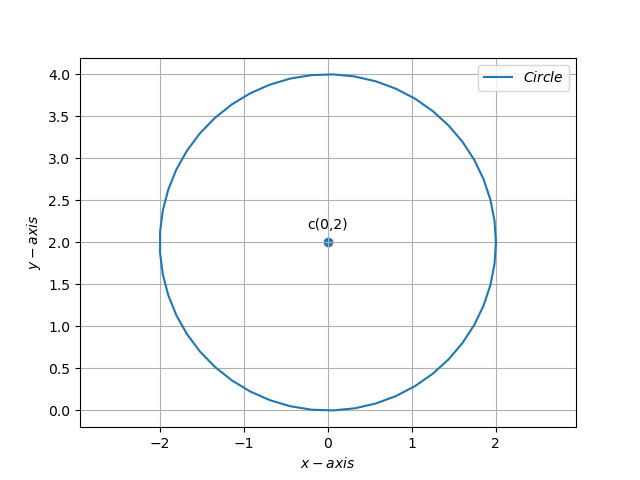
\includegraphics[width=\columnwidth]{chapters/11/11/1/1/figs/circ1}
	\end{center}
\caption{}
\label{fig:11/11/1/1/Fig1}
\end{figure}

